% DEVELOPERNOTE: I am not experienced in the tex language - my approach has been to use basic conditionals and primitives to learn the TeX more.
\section{Hvordan det er at være med i Coding Pirates}
\begin{frame}
\frametitle{Demo og hvordan en game engine ser ud!}
Et produkt fra gamedevafdelingen, som man kan finde på steam!
\begin{figure}
    \href{https://store.steampowered.com/app/1589450/Frogiee/}{\includegraphics[width=\textwidth, keepaspectratio]{/home/madshebsgaard/Projects/CodingPiratesOutReach/assets/pictures/Frogiee_1920x1080.jpg}}
    \caption{Platformerspillet Frogiee af Peter Kragh og Thomas Lauridsen (2021)\cite{Pirates_frogiee}}
    \label{fig:frogiee_screenshot}
\end{figure}
\end{frame}

\begin{frame}
\frametitle{Hvad laver vi? (i GameDev)}
    \newcommand{\gamedevconcepts}{
        Engine, Logik, Assets, Design, Historiefortælling, Samarbejde
    }
    \begin{center}
    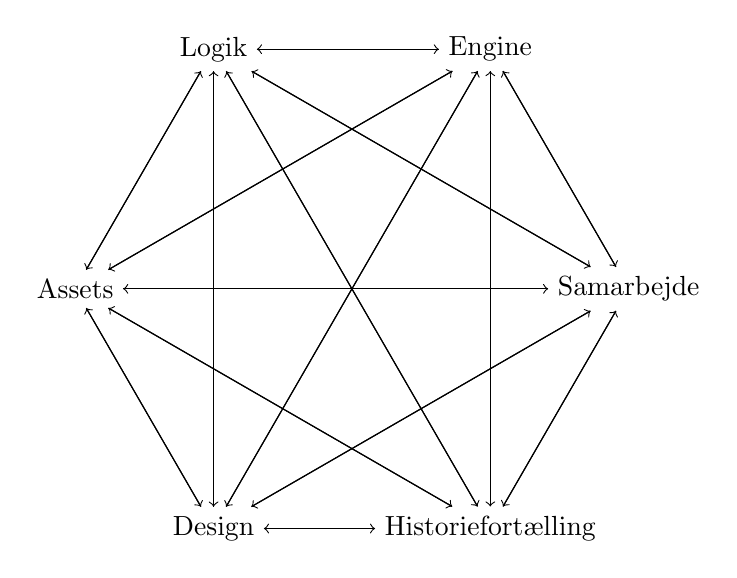
\begin{tikzpicture}
        % Draw boxes (Vertices/Nodes)
        \foreach [count=\i] \x in \gamedevconcepts{
            \node (\x) at(\i*60:10em) {\x};
        }
        % Draw box connects (Edges) 
        \foreach \x in \gamedevconcepts{
            \foreach \y in \gamedevconcepts{
                \ifx\x\y
                    % Don't create loop on every node 
                \else
                    \draw[->] (\x) -> (\y);
                \fi
            }
        }
    \end{tikzpicture}
    \end{center}
\end{frame}

\begin{frame}
\frametitle{Hvordan kan man være med?}
    % Use pseudopredicates to explain how to join coding pirates
    \newcommand{\applicationpredicates}{
        RigtigAlder(x) = $x>=12$år OG $x<= 17$år, 
        InteresseretIComputerSpil(x),
        FriOnsdagAften(x),
        ErNysgerrigPåSoftware(x), 
        KanTilmeldeDig(x) = Har500kr(x) OG KanFindeCodingPirates.dk(x), 
        MedlemAfPiraterne(x),
    }

    Lad x være dig!
    \begin{center}
        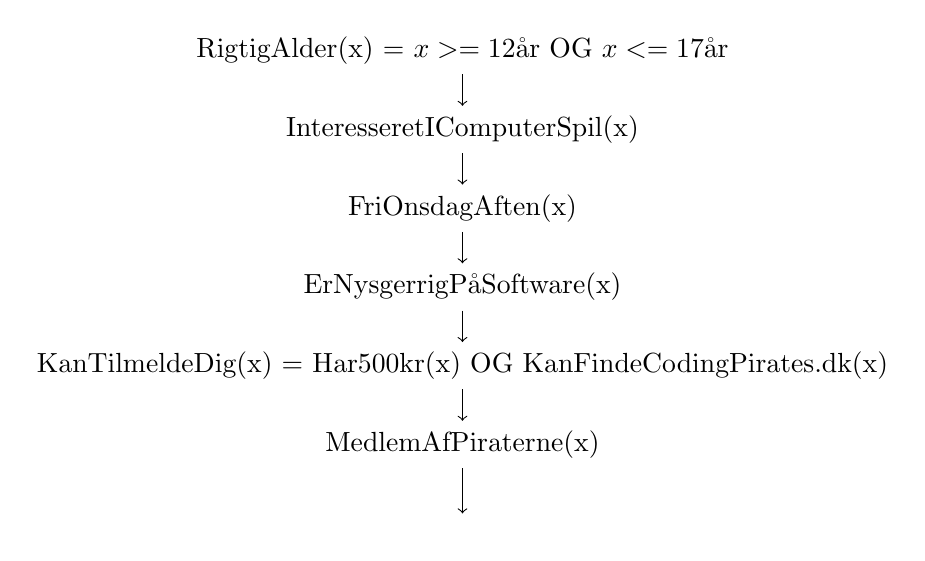
\begin{tikzpicture}
            \foreach [count=\i, remember=\i as \prev (initially dummy)] \x in \applicationpredicates{
                \node (\i) at (0,-\i) {\x};
                \ifnum\i>1
                        \draw[->] (\prev) -- (\i);
                \fi
            }
        \end{tikzpicture}
    \end{center}
\end{frame}


